\documentclass{article}

\usepackage{amsmath,amssymb,amsthm} % Advanced math typesetting
\usepackage[utf8]{inputenc} % Unicode support
\usepackage{tikz}
\usetikzlibrary{shapes.geometric, arrows, calc, svg.path}

\usepackage{hyperref} % Add a link to your document
\hypersetup{
    colorlinks,
    citecolor=blue,
    filecolor=black,
    linkcolor=blue,
    urlcolor=blue
}
\usepackage{graphicx} % Add pictures to your document
\usepackage{listings}
\usepackage{geometry}
\geometry{
 a4paper,
 total={170mm,257mm},
 left=20mm,
 top=20mm,
}
\usepackage{titling}
\usepackage{fancyhdr}
\fancypagestyle{plain}{%  the preset of fancyhdr 
    \fancyhf{} % clear all header and footer fields
    %\fancyfoot[R]{\includegraphics[width=2cm]{KULEUVEN_GENT_RGB_LOGO.png}}
    \fancyfoot[L]{\thedate}
    \fancyhead[L]{SPR200 Basic Cryptography}
    \fancyhead[R]{\theauthor}
}
\usepackage{cmbright}

\title{Lab-02: Describe Cryptographic Protocols \\ with Diagrams and Flowcharts}
\author{Rabbi Muhammad Aman}
\date{\today}

\makeatletter
\def\@maketitle{%
  \newpage
  \null
  \vskip 1em%
  \begin{center}% 
  \let \footnote \thanks
    {\LARGE \@title \par}% 
    \vskip 1em%
  \end{center}%
  \par
  \vskip 1em}
\makeatother

\begin{document}

\maketitle

\noindent\begin{tabular}{@{}ll}
    Student Name & Rabbi Muhammad Aman\\
    Course Code & SPR200\\
    Section Number & NBB \\ 
    Professor & Prof. Wei Huang 
\end{tabular}

\newpage

\section{Practicing Flowchart}
\dots
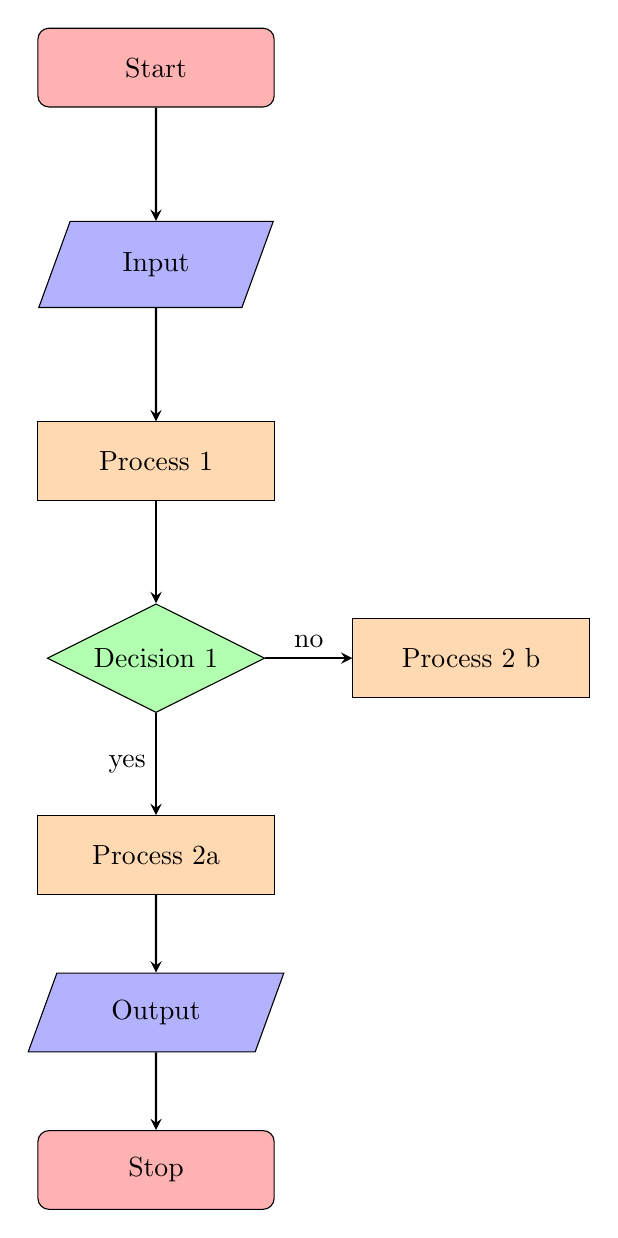
\begin{tikzpicture}[node distance=2cm]
\tikzstyle{start} = [rectangle, rounded corners, minimum width=3cm, minimum height=1cm,text centered, draw=black, fill=red!30]
\tikzstyle{io} = [trapezium, trapezium left angle=70, trapezium right angle=110, minimum width=3cm, minimum height=1cm, text centered, draw=black, fill=blue!30]
\tikzstyle{process} = [rectangle, minimum width=3cm, minimum height=1cm, text centered, draw=black, fill=orange!30]
\tikzstyle{decision} = [diamond, aspect=2, minimum width=2cm, minimum height=0.5cm, text centered, draw=black, fill=green!30]
\tikzstyle{arrow} = [thick,->,>=stealth]
  \node (start) [start] { Start };
  \node (in1) [io, below of=start, yshift=-0.5cm] { Input };
  \node (pro1) [process, below of=in1, yshift=-0.5cm] { Process 1};
  \node (dec1) [decision, below of=pro1, yshift=-0.5cm] { Decision 1};
  \node (pro2a) [process, below of=dec1, yshift=-0.5cm] { Process 2a};
  \node (pro2b) [process, right of=dec1, xshift=2cm] { Process 2 b };
  \node (out1) [io, below of=pro2a] { Output };
  \node (stop) [start, below of=out1] { Stop };
  \draw [arrow] (start) -- (in1);
  \draw [arrow] (in1) -- (pro1);
  \draw [arrow] (pro1) -- (dec1);
  \draw [arrow] (dec1) -- node[anchor=east] {yes} (pro2a);
  \draw [arrow] (dec1) -- node[anchor=south] {no} (pro2b);
  \draw [arrow] (pro2a) -- (out1);
  \draw [arrow] (out1) -- (stop);
\end{tikzpicture}

\newpage

\section{Rainbow Attack Flowchart}

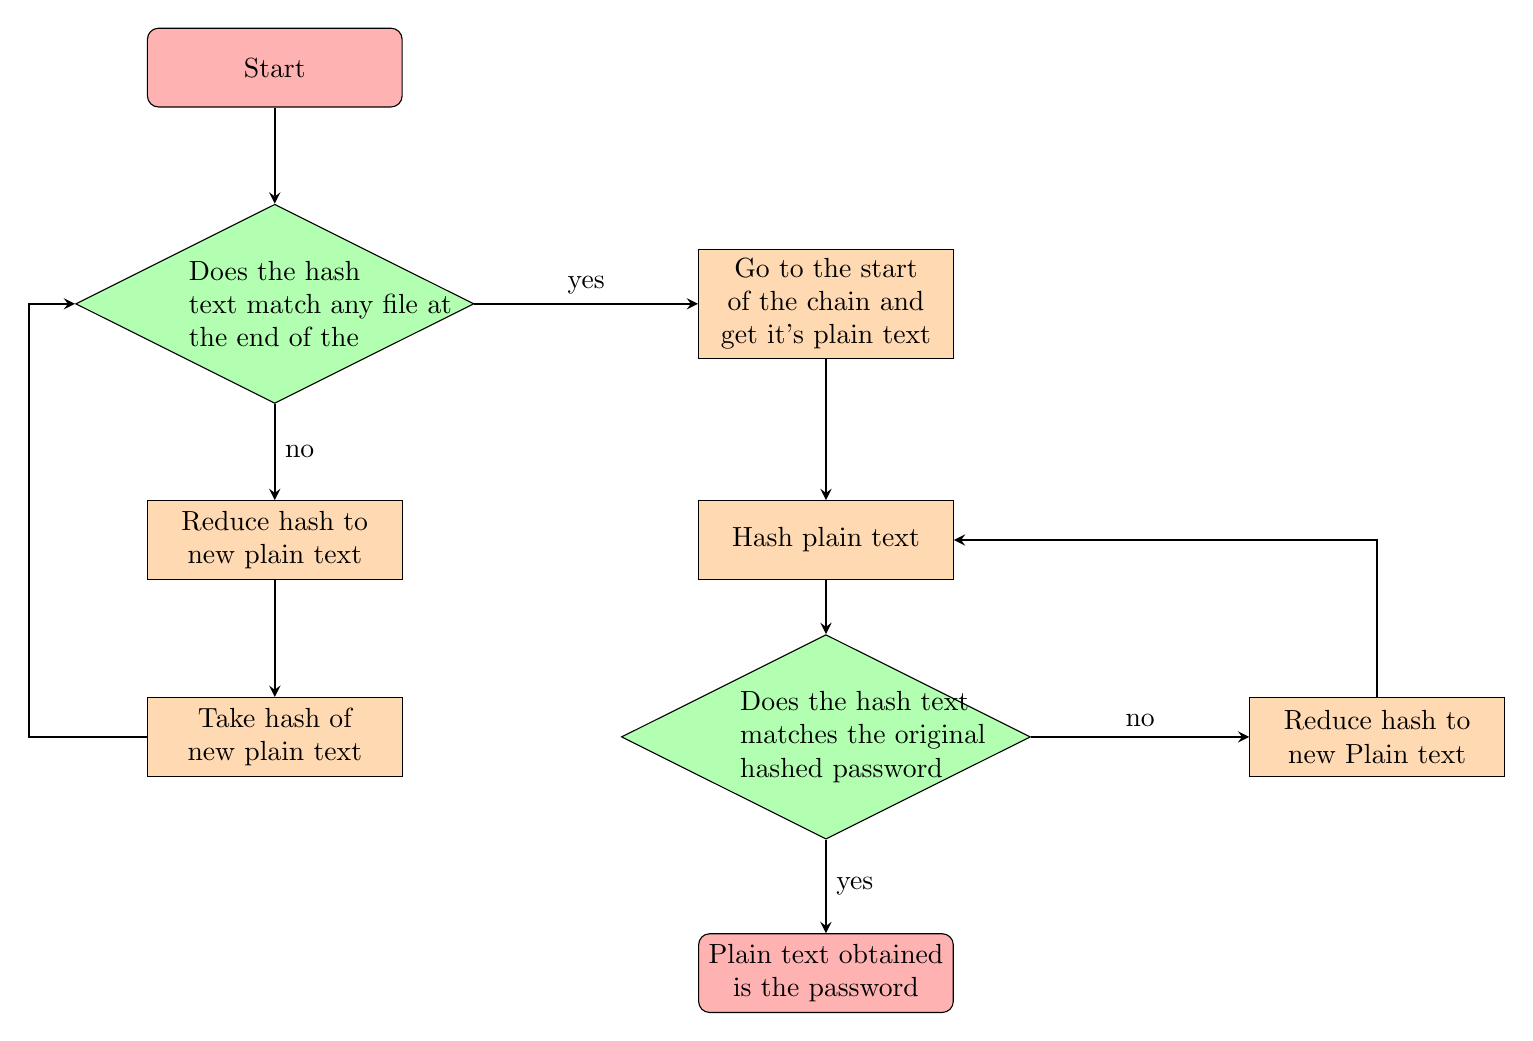
\begin{tikzpicture}[node distance=2cm, every node/.style={align=center}]
  \tikzstyle{start} = [rectangle, rounded corners, minimum width=3cm, minimum height=1cm,text centered,text width=3cm, draw=black, fill=red!30]
  \tikzstyle{io} = [trapezium, trapezium left angle=70, trapezium right angle=110, minimum width=3cm, minimum height=1cm, text centered, draw=black, fill=blue!30]
  \tikzstyle{process} = [rectangle, minimum width=3cm, minimum height=1cm, text centered, text width=3cm, draw=black, fill=orange!30]
  \tikzstyle{decision} = [diamond, aspect=2, minimum width=2cm, minimum height=2cm, text width=2.18cm, draw=black, fill=green!30]
  \tikzstyle{arrow} = [thick,->,>=stealth]
  \node (start) [start, xshift=0cm] { Start };
  \node(diamond) [decision, below of=start, yshift=-1cm] {\vbox{\hbox{Does the hash}\hbox{text match any file at}\hbox{the end of the}}}; 
  \node (pro1) [process, below of=diamond, yshift=-1cm] { Reduce hash to new plain text};
  \node (pro3) [process, right of=diamond, xshift=5cm, text width=3cm] { Go to the start of the chain and get it's plain text};
  \node (pro2) [process, below of=pro1, yshift=-0.5cm] { Take hash of new plain text};
  \node (pro4) [process, right of=pro1, xshift=5cm] { Hash plain text};
  \node(dec2) [decision, right of=pro2, xshift=5cm] {\vbox{\hbox{Does the hash text}\hbox{matches the original}\hbox{hashed password}}};
  \node(pro5) [process, right of=dec2, xshift=5cm] { Reduce hash to new Plain text};
  \node (last) [start, below of=dec2, yshift=-1cm] { Plain text obtained is the password };
  \draw [arrow] (start) -- (diamond);
  \draw [arrow] (diamond) -- node[anchor=west] {no} (pro1);
  \draw [arrow] (diamond) -- node[anchor=south] {yes} (pro3);
  \draw [arrow] (pro1) -- (pro2);
  \draw [arrow] (pro3) -- (pro4);
  \draw [arrow] (pro4) -- (dec2);
  \draw [arrow] (dec2) -- node[anchor=south] {no} (pro5);
  \draw [arrow] (dec2) -- node[anchor=west] {yes} (last);
  \draw [arrow] (pro5) |- (pro4);
  \draw [arrow] (pro2.west) -| ++(-1.5cm, 0cm) |- (diamond.west);
\end{tikzpicture}

\newpage

\section{Hash Function Properties Diagram}

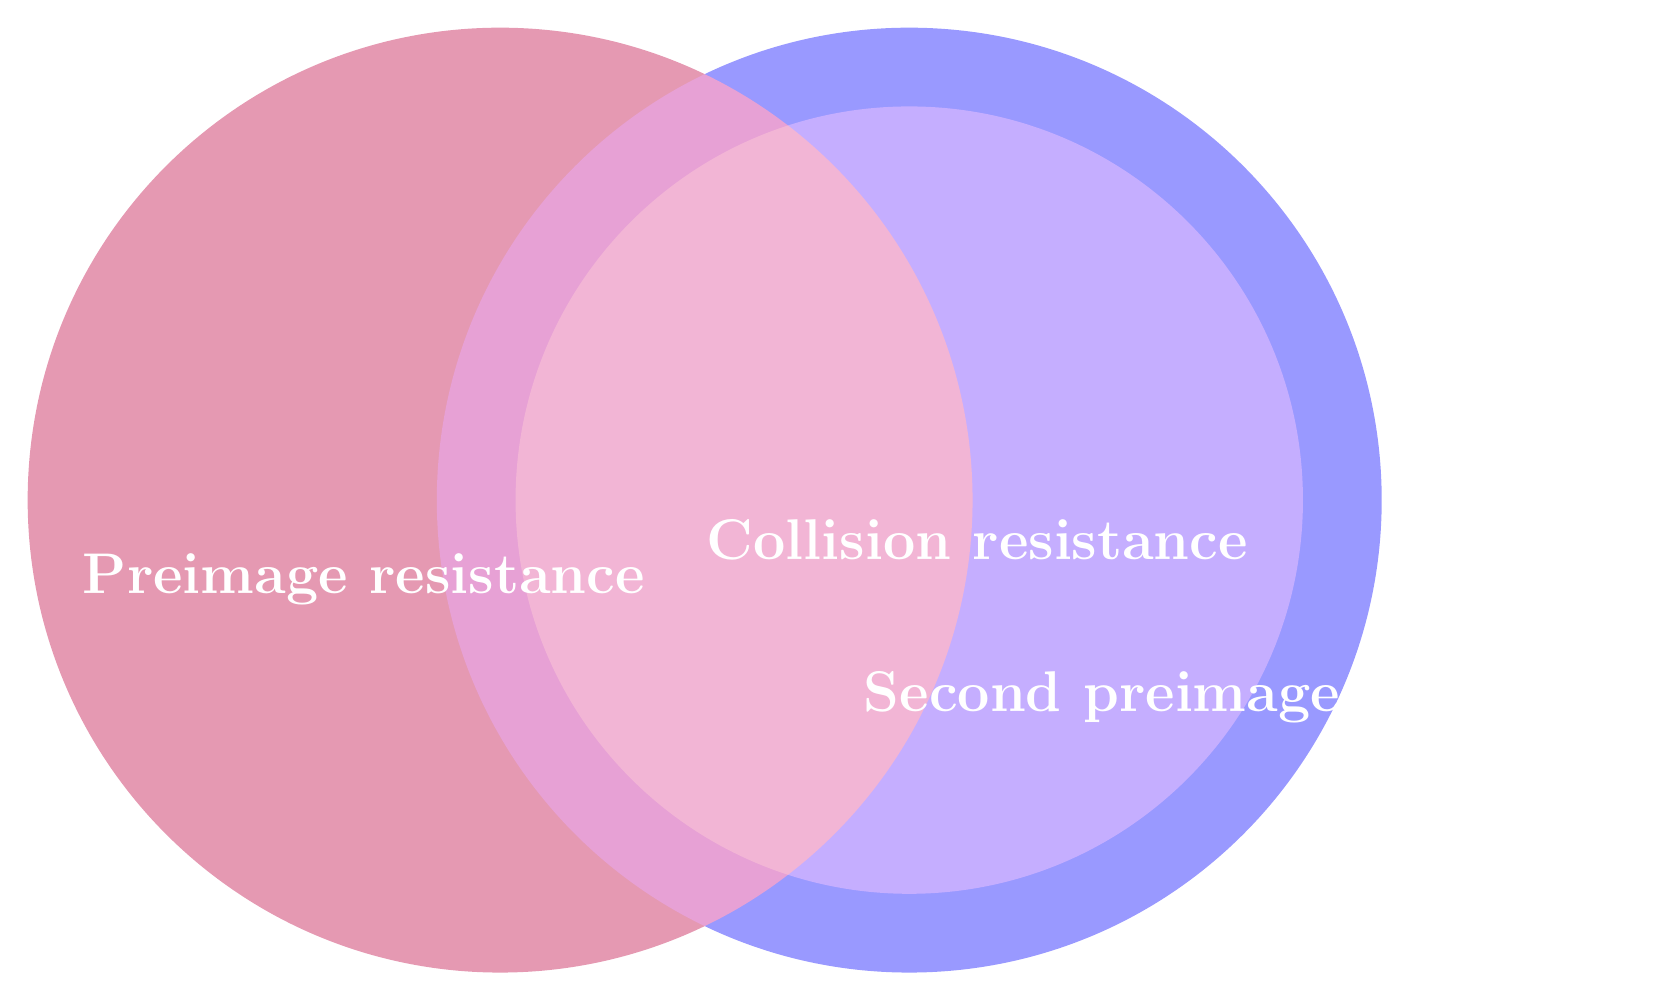
\begin{tikzpicture}
\begin{scope}[blend group=soft light]
% Updated colors and size for the circles
\fill [purple!40!white] (210:3) circle (6); % Increased size and changed color
\fill [blue!40!white] (330:3) circle (6); % Increased size and changed color
\fill [orange!50!white] (330:3) circle (5); % Increased size and changed color
\end{scope}
% Updated text color and size
\node at (210:5) {\huge \textbf{\textcolor{white}{Preimage resistance}}}; % Increased font size and changed color
\node at (330:8) {\huge \textbf{\textcolor{white}{Second preimage resistance}}}; % Increased font size and changed color
\node at (330:4) {\huge \textbf{\textcolor{white}{Collision resistance}}}; % Increased font size and changed color
\end{tikzpicture}

\newpage

\section{Remote Coin-Flipping Protocol with One-Way Function}
\subsection{Draw an illustration of the protocol based on the lecture}
\begin{center}
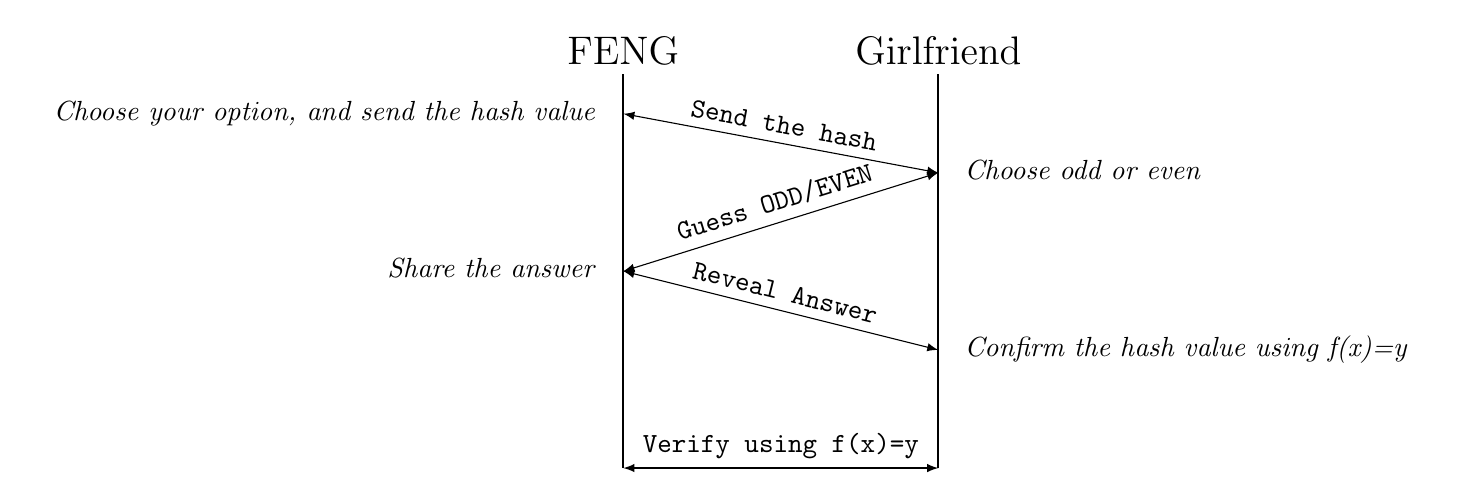
\begin{tikzpicture}[>=latex]
\coordinate (A) at (2.5,5.5);
\coordinate (B) at (2.5,0.5);
\coordinate (C) at (6.5,5.5);
\coordinate (D) at (6.5,0.5);
\draw [thick] (A) -- (B) (C) -- (D);
\draw (A) node [above] {\Large FENG};
\draw (C) node [above] {\Large Girlfriend};
\coordinate (E) at ($(A)!.1!(B)$);
\draw (E) node [left] {\begin{tabular}{r}
\textit{Choose your option, and send the hash value}\\
\end{tabular}};
\coordinate (F) at ($(C)!.25!(D)$);
\draw (F) node [right] {\begin{tabular}{l}
\textit{Choose odd or even}
\end{tabular}};
\draw [<->] (E) -- (F) node [midway, sloped, above] {\verb$Send the hash$};
\coordinate (G) at ($(A)!.5!(B)$);
\draw (G) node [left] {\begin{tabular}{l}
\textit{Share the answer}\\
\end{tabular}};
\draw [<->] (F) -- (G) node [midway, sloped, above] {\verb$Guess ODD/EVEN$};
\coordinate (H) at ($(C)!.5!(D)$);
\draw [<->] (B) -- (D) node [midway, above] {\verb$Verify using f(x)=y$};
\coordinate (I) at ($(A)!.7!(B)$);
\coordinate (J) at ($(C)!.7!(D)$);
\draw (J) node [right]  {\begin{tabular}{l}
\textit{Confirm the hash value using f(x)=y}\\
\end{tabular}};
\draw [<->] (G) -- (J) node [midway, sloped, above] {\verb$Reveal Answer$};
\end{tikzpicture}
\end{center}

\subsection{Explain this cryptographic protocol}

This protocol uses a hash function to ensure that there is no cheating between Feng and his girlfriend. The protocol begins with Professor Feng and his girlfriend deciding on what to eat. They decide to use a remote coin flip to decide whose dinner choice will be selected today. Feng first guesses a number and asks his girlfriend to guess whether it is odd or even. Next, his girlfriend decides on her number and replies to Feng. Since they are not together in person, Feng cannot cheat, and his girlfriend insists that she would not like that. To prevent this, Feng already created the equation \(f(x) = y\) and gave the value of \(y\) to his girlfriend. All she needs to do is verify her answer by plugging her value for \(x\) into the equation. If the value of \(y\) is correct, the hash value provided by Feng is valid. If the value of \(y\) is incorrect, Feng was caught cheating, and now he has to eat according to his girlfriend's choice for the rest of his life. The hash provided by Feng guarantees that he did not cheat, and his girlfriend’s choice ensures she didn’t cheat.

\subsection{ why this protocol would work and why neither Professor Feng nor his girlfriend can cheat in this protocol?}

This protocol works remotely because Feng has already provided the answer to the equation \(f(x) = y\). His girlfriend simply needs to input the value of \(x\), which represents the pre-image resistance, and perform the calculation to check if \(y\) holds. If \(y\) matches, the hash value provided by Feng is correct. If \(y\) does not match, Feng’s hash value is incorrect, meaning he cheated. This protocol is secure because Feng has already shared the hash value, and his girlfriend provides the value of \(x\). If either of them cheats, the equation will not be satisfied, and the hash will be invalid.

\end{document}
